\chapter{Résultats}

Dans le chapitre précédent, nous avons vu que des mesures du retournement de l'aimantation étaient facilement identifiables et qu'en outre, elles permettaient de d'identifier les différents états de spin nucléaire du noyau de Terbium.

Nous allons voir maintenant qu'il est possible d'utiliser notre système pour étudier le magnétisme d'une molécule unique afin de le comparé à celui inféré à partir des études en microcristaux. 

De plus, nous montrerons également comment la dynamique du spin nucléaire peut être étudier afin d'accéder au temps de relaxation de ce dernier. De plus, nous mettrons en évidence la dépendence de ce temps de relaxation vis a vis environnement  électrostatique.


Enfin, une étude en température sera présenté mettant en évidence la bonne thermalisation du spin nucléaire.

\section{Aimantation des aimants moléculaires}
Avant de nous consacrer à l'étude d'une molécule isolée, nous allons nous attarder un instant sur les mesures obtenues à l'aide de cristaux moléculaires. L'aimantation en fonction du champ magnétique de ces derniers est obtenue à l'aide d'une mesure micro-SQUID. Lorsque l'aimantation d'un aimant moléculaire change, les lignes de champ qu'il génère change également, entraînant une modification de flux auquel le micro-SQUID est sensible. En amenant d'abord l'aimantation à saturation par l'application d'un fort champ magnétique, puis en balayant celui-ci vers une valeur opposée, on peut remonter à l'aimantation en fonction du champ magnétique. La Fig.??? montre une mesure de ce type dans l'un cas d'un cristal de TbPc$_2$ dilué à 10\%. La dilution est obtenue en insérant des molécules de YPc$_2$ de même structure mais non magnétique.

Dans notre expérience, nous n'avons accès qu'à un seul aimant moléculaire. Il nous faut donc utiliser l'hypothèse ergodique à savoir : mesurer un assemblé de N molécules est équivalent à mesurer $N$ fois la même molécule. Pour le reste, la technique de mesure est identique. L'aimantation est amenée à saturation, ce qui revient, dans notre cas, à appliquer un champ magnétique suffisamment grand pour que l'aimantation de la molécule se retourne. Le champ magnétique est ensuite balayé et la position en champ magnétique du retournement de l'aimantation est relevée. Ce cycle est effectué $N$ fois afin de pouvoir constituer une statistique~(dans nos expérience, $N$ à pris des valeur entre 1000 et 22000 selon les cas). L'aimantation est ensuite reconstitué. Pour cela on note $\mathscr{N}(B)$ le nombre de molécules s'étant retournées avant le champ magnétique $B$ et on attribue le moment magnétique $\frac{M_s}{N}$ à chaque molécule, $M_s$ étant l'aimantation de saturation et $N$ le nombre total de mesures. L'aimantation en fonction du champ magnétique prend alors la forme suivante :
\begin{eqnarray}
M(B) =\pm \frac{M_s}{N}(2\mathscr{N}(B) -1)\nonumber
\end{eqnarray}

Le signe est déterminé par celui du champ magnétique du champ de saturation initial : positif pou un champ de saturation est négatif; négatif pour un champ de saturation positif. Pour une comparaison plus aisée avec les mesure micro-SQUID, on peut ré-exprimer la formule précédente comme suit :
\begin{eqnarray}
\frac{M}{M_s}(B) =\pm \frac{1}{N} (2\mathscr{N}(B) -1)
\end{eqnarray}

Le résultat obtenue pour un champ de saturation de $\pm 400 \, mT$, une vitesse de balyage de $50\,mT.s^{-1}$ et pour $N$ mesures, est présentée dans la Fig??.

Afin de faciliter la comparaison des deux mesures, j'ai choisi de diviser la mesure en trois zone : champ faible pour $|B|< 100\,mT$, champ moyen pour $100\,mT<|B|< 200\,mT$ et champ fort pour $|B| > 200\,mT$.

A faible champ, la structure en marche caractéristique du phénomène de QTM~\cite{Thomas1996,Friedman1996} est clairement visible dans les deux mesures comme le montre la Fig?? et l'agrandissement dans la Fig??. Une différence notable réside cependant dans le nombre de marches observées. Alors que dans nos mesures, seulement 4 marches sont présentes~(conformément aux prédictions théoriques), le mesure obtenues à l'aide d'un cristal moléculaire montre de nombreuses marches supplémentaires. Ces dernières sont très certainement induites par des interactions entre les différents centres magnétique du cristal~\cite{Wernsdorfer2002}, et ce, malgré la dilution à 10\%.

A champ moyen, les deux mesures diffèrent largement. Dans le cas des mesures micro-SQUID, le retournement de l'aimantation est continue et les marches observés à faible champ sont totalement absentes. Dans cette zone, le retournement est induit par le bain de phonons et non par un phénomène de QTM. Dans le cas de l'aimant moléculaire isolé, on observe une deuxième série de quatre marches similaires à celles obtenues dans le cas du QTM. L'évolution de ces transitions en fonction du champ transverse nous laisse penser que celles-ci sont d\^u à un couplage entre l'aimant moléculaire et un deuxième système magnétique. De plus, le couplage avec le bain de phonons, présent dans le cas d'un cristal moléculaire, est ici absent. Ceci peut s'expliquer par la petit taille du système ne permettant pas la présence de phonons aux énergies correspondantes au champ magnétique de la zone de champ moyen.

A champ fort là encore, les différences sont notables : retournement assisté par le bain de phonons dans le cas du cristal moléculaire; presence  de marches supperposé à un retournement continue dans le cas de notre système. Ne disposant pas, pour le moment, de modèle expliquant ces caractéristiques, nous ne nous attarderons pas sur cette dernière partie du cycle d’hystérésis et nous de développerons une analyse détaillée que de la zone champ faible.

\section{Dynamique du spin nucléaire}

\subsection{Temps de relaxation du spin nucléaire}
Le spin nucléaire, du fait de son couplage relativement faible à l'environement, possède généralement un temps de vie élevé. Afin de pouvoir vérifier cette propriété, il nous faut pouvoir mesurer l'évolution des états du spin nucléaire en fonction du temps. Nous avons choisi pour cela une technique simple consistant à mesurer l'état du spin nucléaire lors de deux mesures, en faisant varier le temps séparant ces dernières. Du fait de l'aspect chronophage de cette procédure~(jusqu'à plusieurs jours par mesure), nous avons choisi cinq temps d'attente différents : $0,5,10,20$ et $50$ secondes. Pour chacune de ces valeurs, $22000$ balayges ont été effectués afin d'obtenir une statistique significative.


\begin{figure}
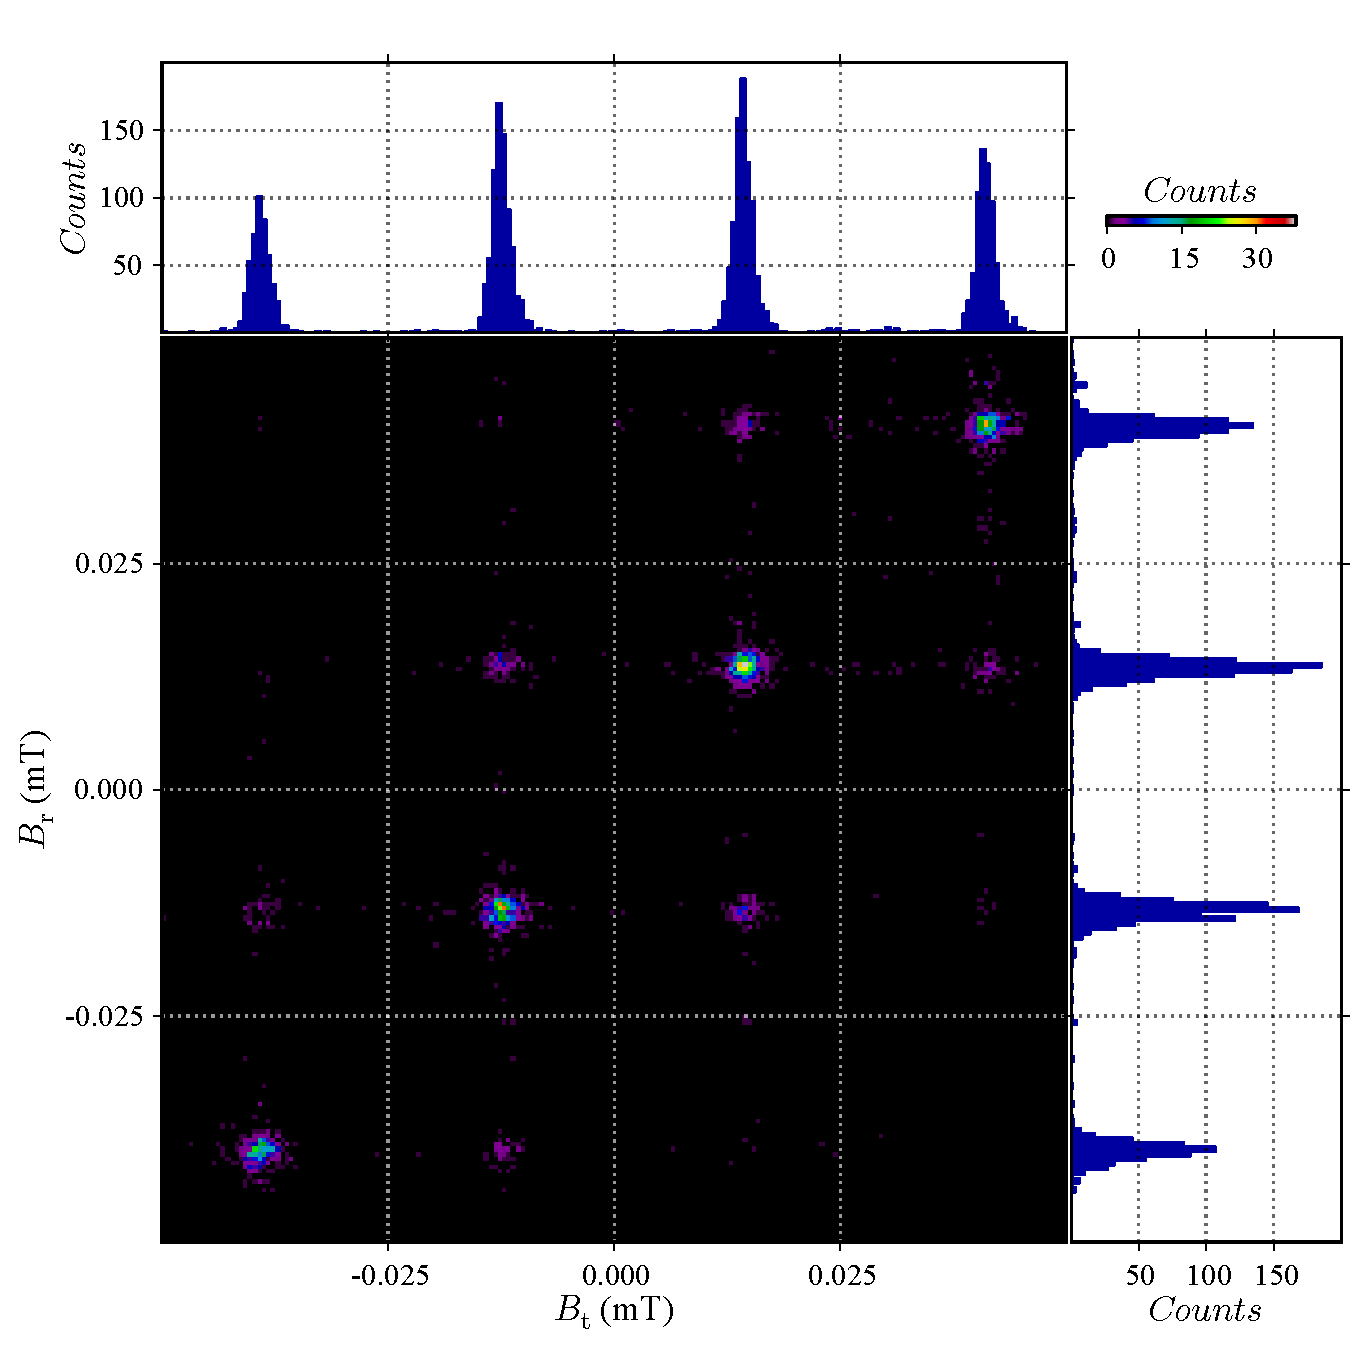
\includegraphics[scale=0.45]{Resultats/Chap2/Figure1/figure1.pdf} 
\caption{La cartographie couleur en deux dimensions représente l’histogramme de corrélation entre la position en champ magnétique des retournements ayant lieu durant la trace et la retrace.Celui-ci a été obtenu à partir de 22000 traces et retraces mesurées consécutivement et sans temps d'attente. Les histogramme à une dimension disposé le long des axes x et y représente respectivement les positions en champ magnétique des retournement durant la trace et la retrace. La prépondérance des éléments diagonaux atteste de la préservation de l'état de spin entre deux mesures.}
\label{correlations}
\end{figure}

L'évolution des états du spin nucléaire est représenté à l'aide d'un histogramme à deux dimensions. Le champ de retournement de la première mesure est repéré en abscisse et celui mesuré lors de la seconde mesure est représentée en ordonnée. Dans une telle représentation, les éléments diagonaux rendent compte d'un état de spin nucléaire qui ne change pas entre les deux mesures. Les éléments hors-diagonaux représente quant à eux las cas où l'état de spin nucléaire varie de $\Delta m_z^I = \pm 1,2,3$ où $m_z^I$ est la projection du moment angulaire du spin nucléaire sur l'axe $z$. La Fig.\ref{correlations} présente une telle mesure pour un temps d'attente nul. Pour faciliter la lecture, l'histogramme des champs de retournement de la première et deuxième mesures a été ajouté.

La Fig.\ref{evolution_temps} montre l'évolution de l'histogramme en fonction du temps d'attente entre les deux mesures. Les éléments diagonaux dominent jusqu'à un temps d'attente de $20$ secondes, prouvant que le spin nucléaire demeure majoritairement inchangé sur ce laps de temps. En revanche, pour un temps d'attente de $50$ secondes, on constate que les éléments diagonaux ne sont plus prépondérant signifiant le perte de l'état nucléaire entre les deux mesures. De plus, la résonance correspondant à l'état de spin $|-3/2 \rangle$ domine largement. Cela traduit la tendance du système à évoluer vers l'équilibre thermodynamique lorsque le temps d'attente devient trop élevé. Nus reviendrons sur ce dernier point dans la suite.

\begin{figure}[h]
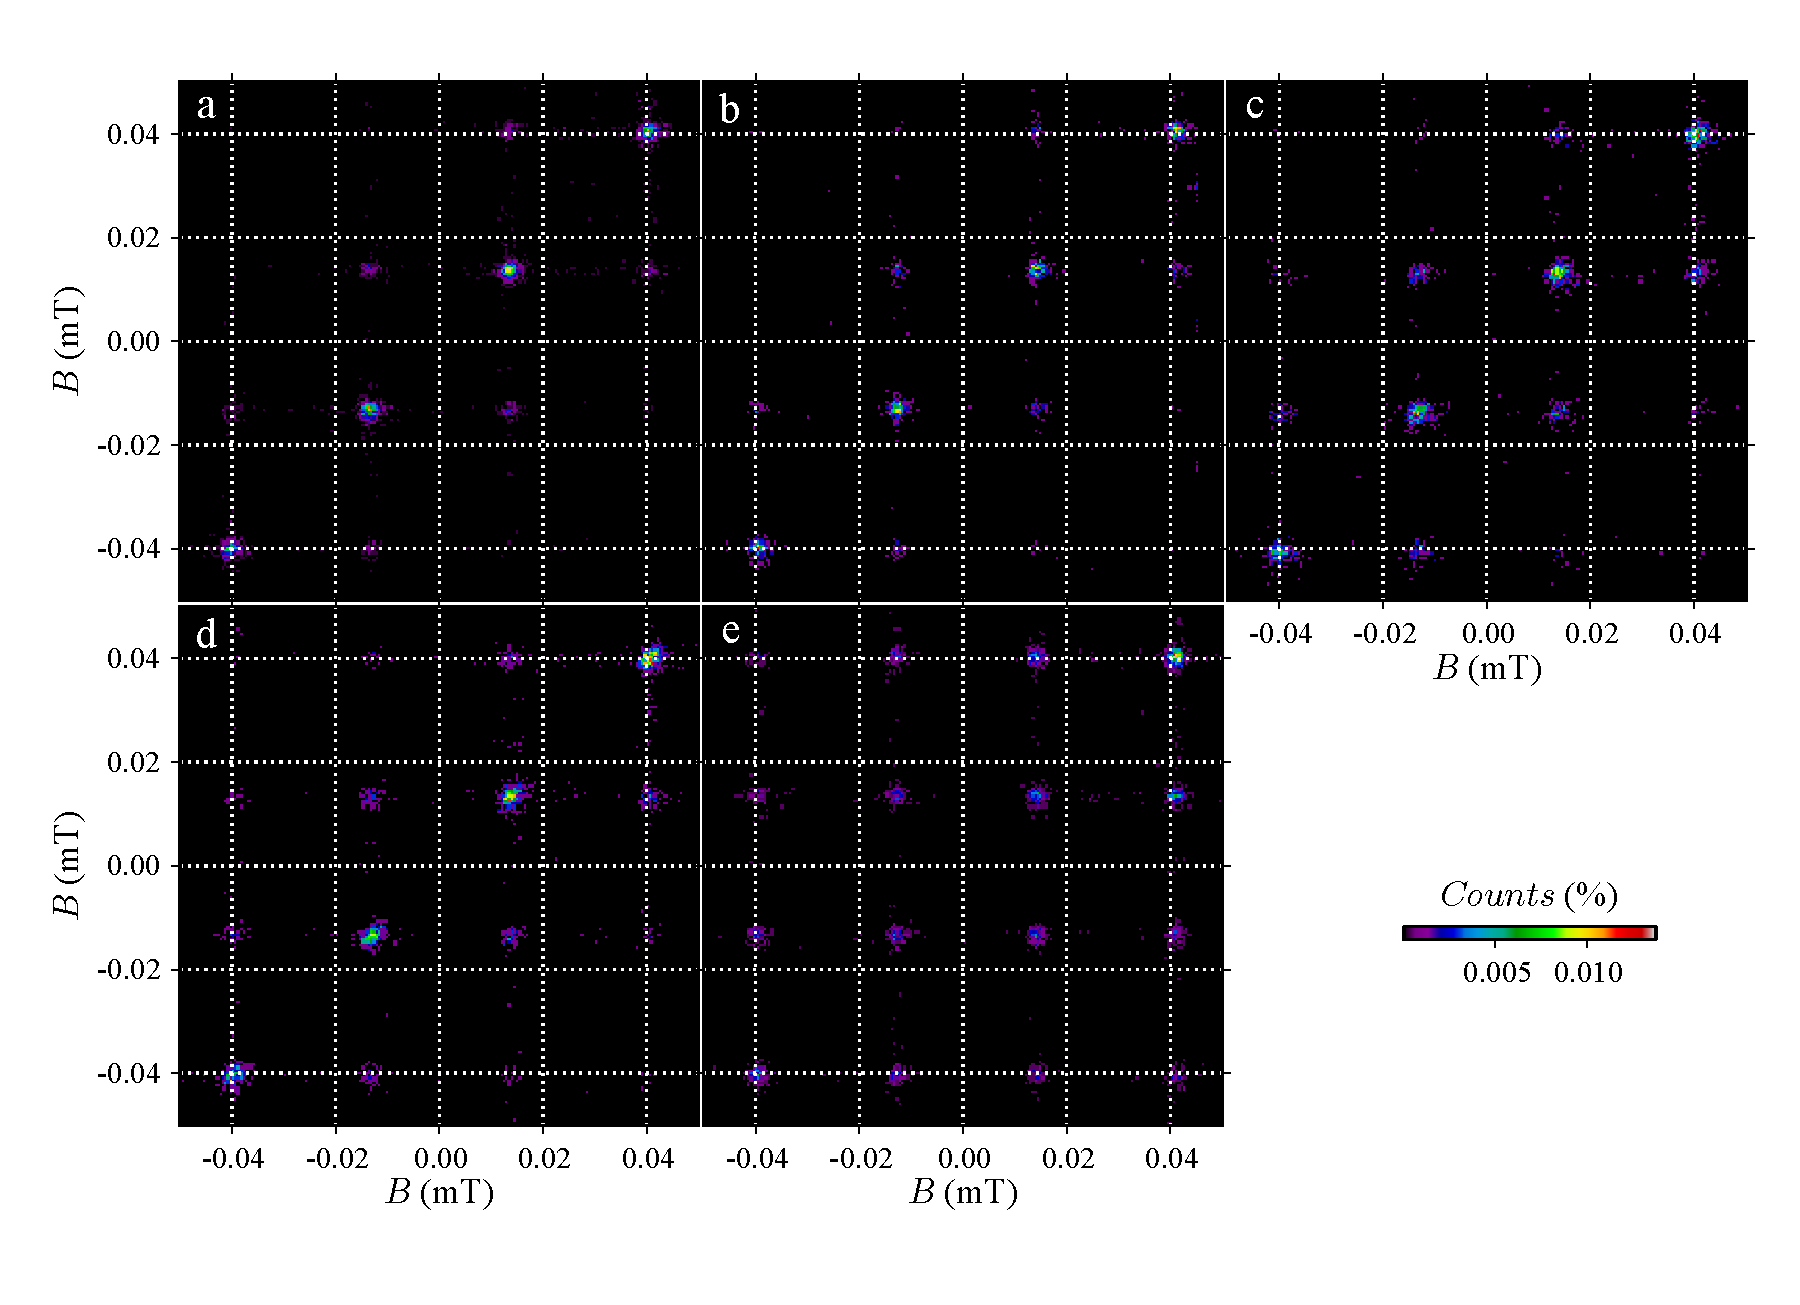
\includegraphics[scale=0.45]{Resultats/Chap2/Figure2/figure2.pdf} 
\caption{La cartographie a (b, c, d et e) présente un histogramme 2D rendant compte de la corrélation entre deux mesures obtenues durant la trace et la retrace, ces dernières étant séparé d'un temps d'attente de 0 secondes (5, 10, 20 et 50 secondes). La prédominance des élements diagonnaux pour des temps d'attente allant au-delà de la dizaine de seconde démontre le long temps de vie des états du spin nucléaire.}
\label{evolution_temps}
\end{figure}


\subsection{Perturbations induites par la mesure}
De m\^eme que nous pouvons étudier l'influence du temps d'attente sur le spin nucléaire, il peut \^etre intéressant d'évaluer l'influence de la mesure sur l'état de spin nucléaire. Pour cela, nous avons choisi d'utiliser la méthode présenté précédemment, en observant non plus l'évolution de l'état nucléaire en fonction du temps mais en fonction du nombre de mesures. Nous avons utilisé les donnée collecté sur 22000 balayages (11000 trace et autant de retrace) effectué sans temps d'attente.

La Fig.\ref{evolution_mesures} présente cette évolution après deux~(\textbf{a}), trois~(\textbf{b}), quatre~(\textbf{c}), cinq~(\textbf{d}) et six~(\textbf{e}) mesures. On constate qu'après 4 mesures, les éléments diagonaux domine toujours, pour ne commencer à s'atténuer qu'au bout de 6 mesures. Il est important de noté que chaque mesure est, en moyenne, séparée de 4 secondes, et donc, dans le cas de 6 mesures, cela correspond à un temps totale de plus de 20 secondes. Aux vues des résultats présentés dans la section précédente, on peut attribuer cette diminution de corrélation dans l'état du spin nucléaire au processus de relaxation interne au système, la procédure de mesure elle-même n'affectant qu'à la marge le système. 

La méthode de mesure de l'état de spin nucléaire par l'intermédiaire du QTM se révèle donc peu invasive, ce qui permet d'étudier les propriétés du système en négligeant son influence sur ce dernier.

\begin{figure}
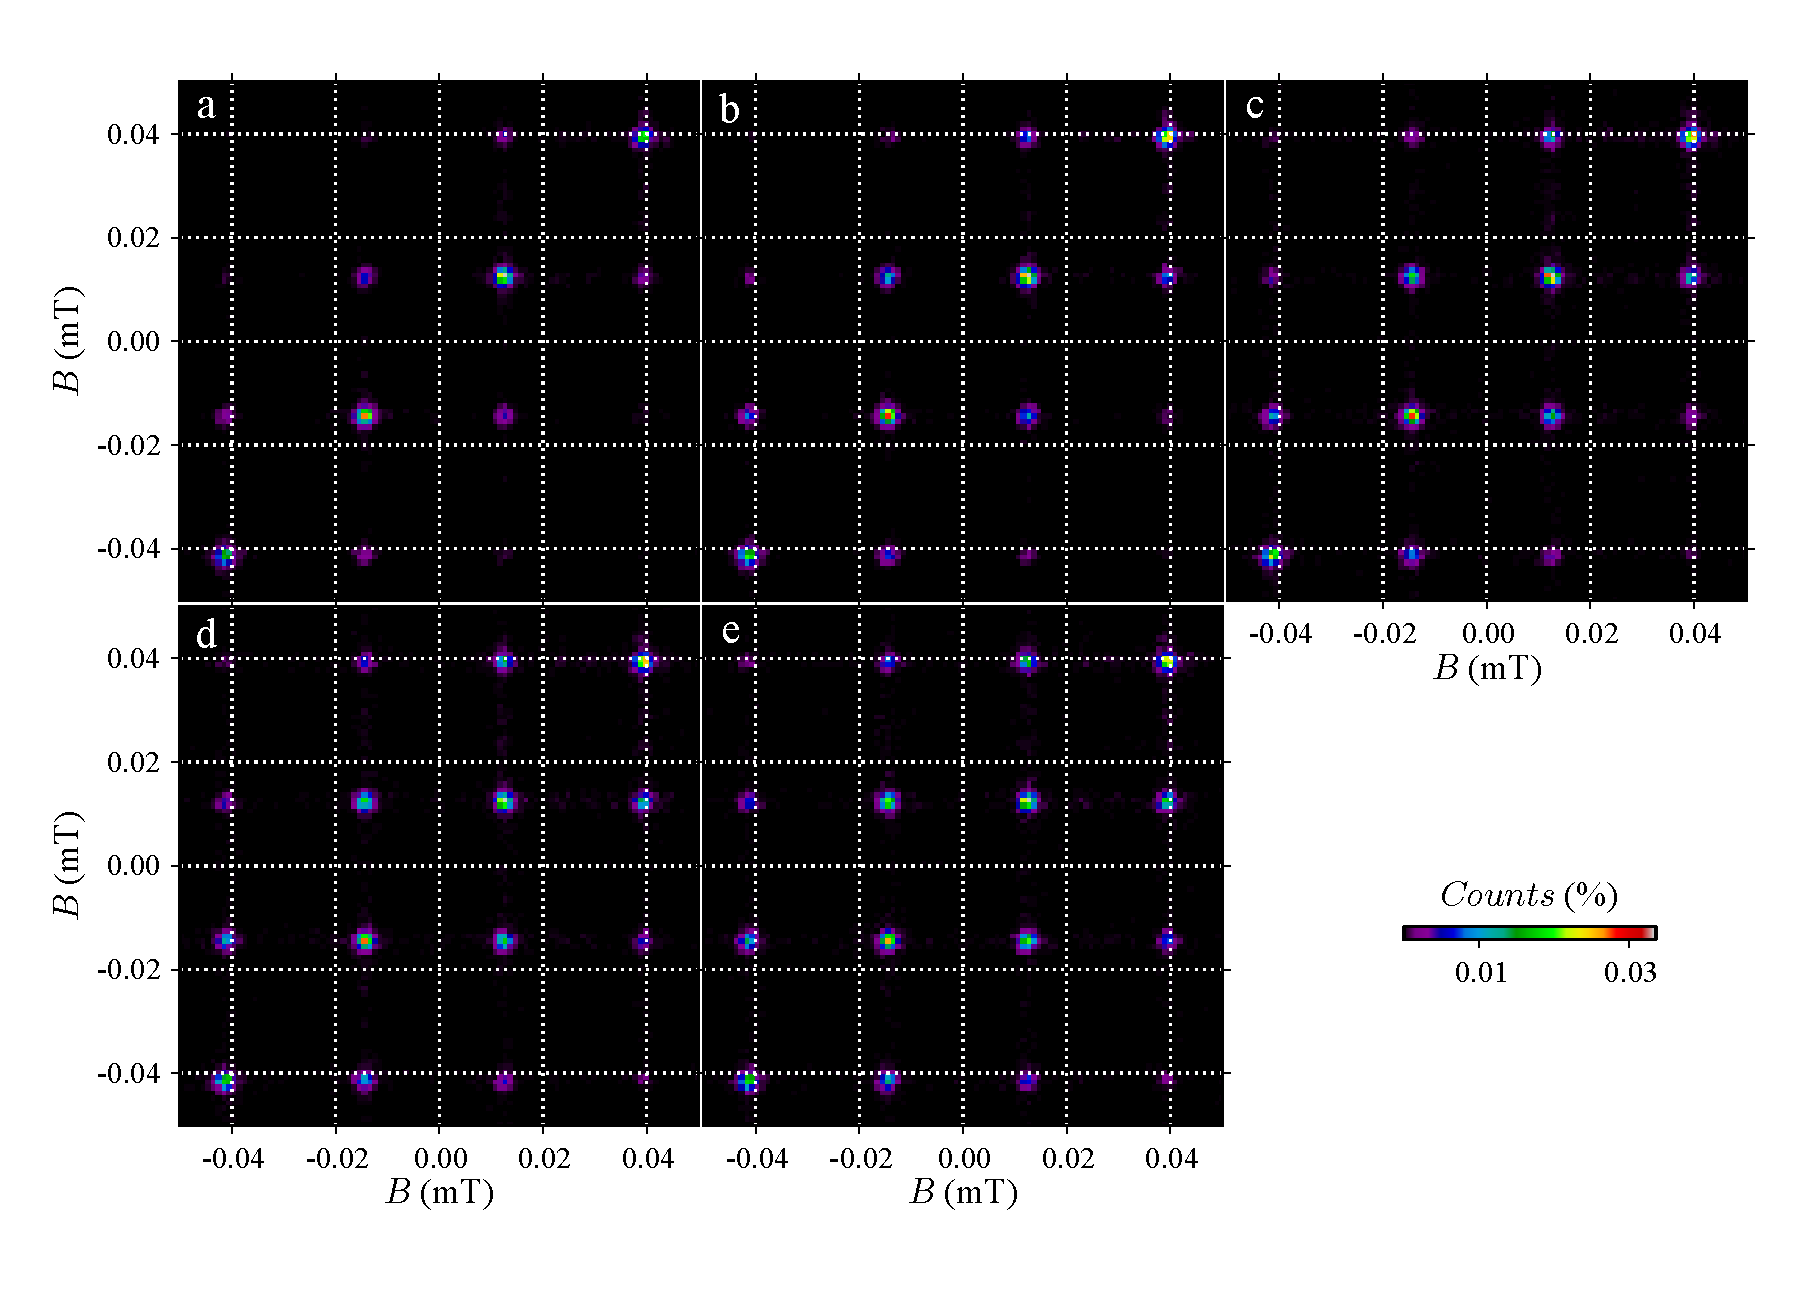
\includegraphics[scale=0.45]{Resultats/Chap2/Figure3/figure3.pdf} 
\caption{La cartographie a (b, c, d et e) présente un histogramme 2D rendant compte de la corrélation entre les états de spin nucléaire après deux (trois, quatre, cinq et six) mesures. On constate qu'après six mesures, les éléments diagonaux sont toujours dominant démontrant ainsi le faible influence de notre procédure de mesure sur l'état du spin nucléaire.}
\label{evolution_mesures}
\end{figure}


\subsection{Extraction de la population des états nucléaires}

Au chapitre précédent, nous avons montré qu'à travers un histogramme des positions en champ des renversements, on pouvait facilement identifier les différents états de spin.Nous allons utiliser cette m\^eme mesure en la présentant différemment. En effet, chaque retournement au voisinage d'une résonance peut \^etre attribuée à un état de spin précis, les différents résonances ne se recouvrant pas. En intégrant et en normalisant le nombre de mesures obtenues pour chaque état de spin nucléaire, on peut reconstruire leur distribution. C'est ce qui est présenté dans la Fig. \ref{extract_pop} ou l'histogramme original est montré en \textbf{a} et la population qui en est extraite en \textbf{b}.

Cependant, cette dernière contient en fait deux distributions, l'une relative à $J_z=-6$ et l'autre à $J_z=+6$ comme nous l'avons déjà montré. Il est cependant possible de les différencié à partir du signe du changement en conductance relatif à chaque mesure $\Delta g$. Dans la suite, du fait d'un initialisation à champ négatif, nous prendrons toujours pour référence la situation où $J_z=-6$ car il s'agit de l'état fondamental, donc plus probable, et il fournis donc une meilleure statistique.

\begin{figure}
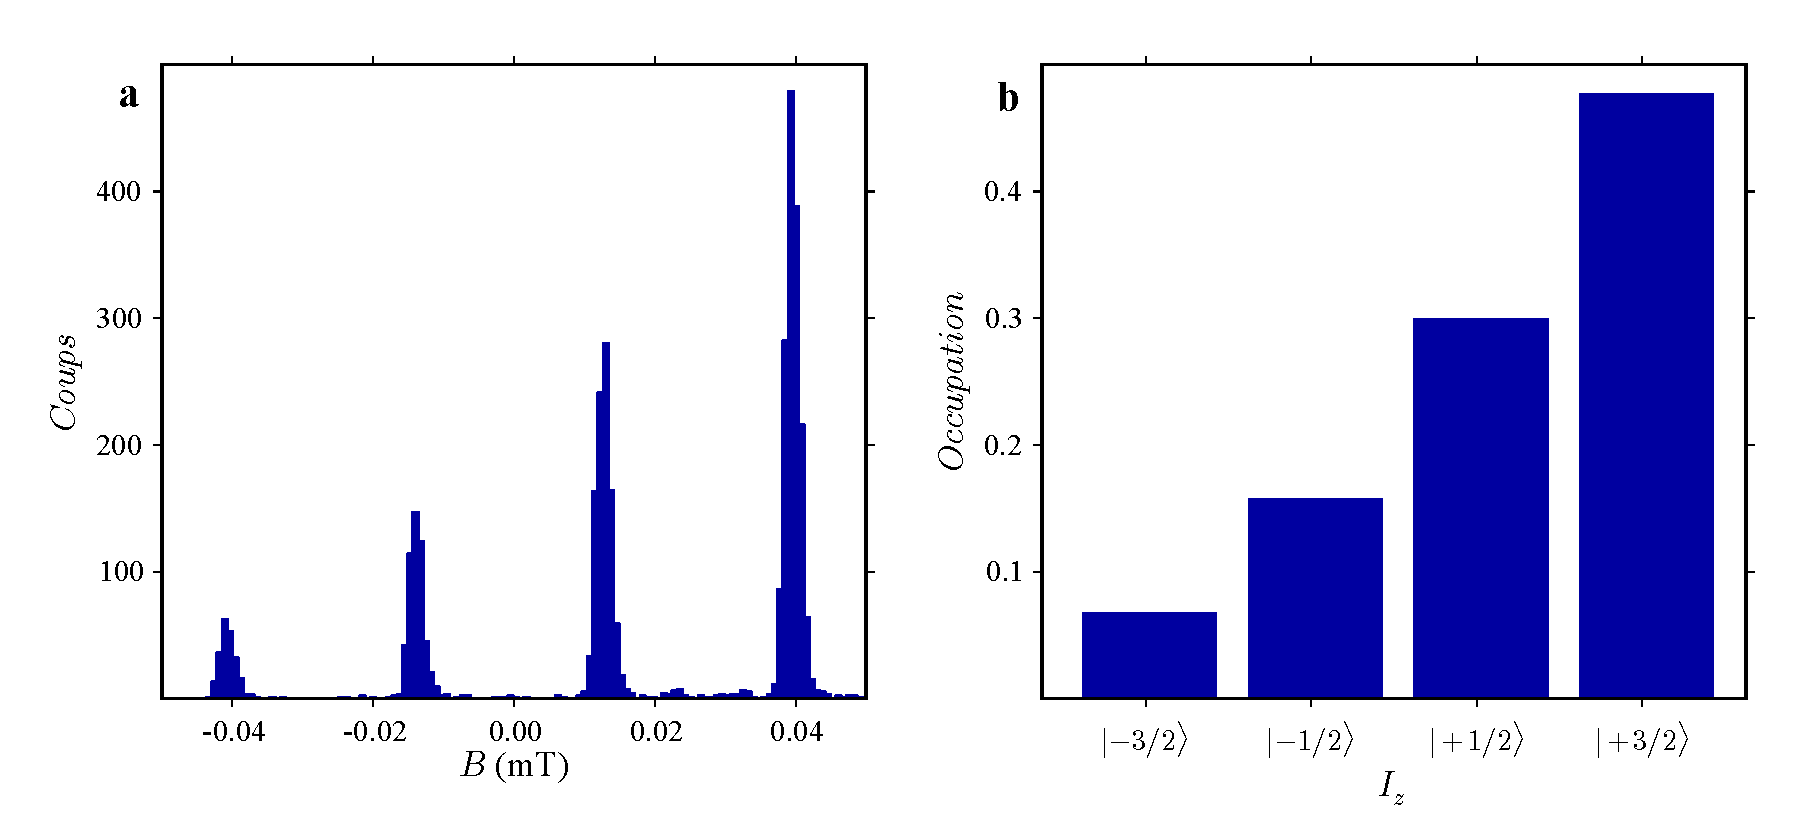
\includegraphics[scale=0.45]{Resultats/Chap2/Figure4/figure4.pdf} 
\caption{\textbf{a -} Histogramme des champs de retournement obtenue durant la trace et correspondant à la transition $J_z = +6 \rightarrow -6$. \textbf{b -} Population des états de spin nucléaire obtenue à partir de l'histogramme présenté en \textbf{a}. Du fait de la relaxation, on constate la prédominance de l'état fondamental $I_z=+3/2$ sur les autres états.}
\label{extract_pop}
\end{figure}

Nous allons maintenant utiliser cette technique d'extraction des populations pour étudier son évolution en fonction du temps pour deux environnements électrostatiques différents.

\subsection{Influence de la tension de grille sur la relaxation}
Afin d'évaluer l'influence de la tension de grille sur la relaxation, nous avons mesuré l'évolution de la population des états de spin en fonction du temps pour deux points polarisation ($V_g$,$V_{ds}$) différent : ($-0.9\, V$,$0\, V$) et ($-0.1\, V$,$0\, V$). Pour chacun de ces points nous avons fait varié le temps d'attente entre la retrace et la trace suivante de 0, 5, 10, 20 et 50 secondes et la population des états nucléaire a été reconstruite à partir des transitions obtenues durant la trace, en sélectionnant seulement celles correspondant à l'état fondamental $J_z=+6$.

La Fig.\ref{dynamique_spin}.\textbf{a} et \textbf{b} présentent les résultats obtenus. On constate immédiatement que les deux distribution évolue différemment. Pour la tension de grille $V_g = -0.9V$ la relaxation vers l'équilibre thermodynamique se fait plus lentement que lorsque $V_g = -0.1V$.  Ceci peut s'expliquer par la modification du courant circulant à travers le système du fait de la modification de la tension de grille. Celle-ci entraîne un changement dans les fluctuations de champ électrique  qui, en se couplant au moment quadripolaire du spin nucléaire, vont modifier les processus de relaxation.

Un analyse plus fine en grille n'a cependant pas permis déterminer le phénomène physique rendant compte de cette dépendance.

\begin{figure}
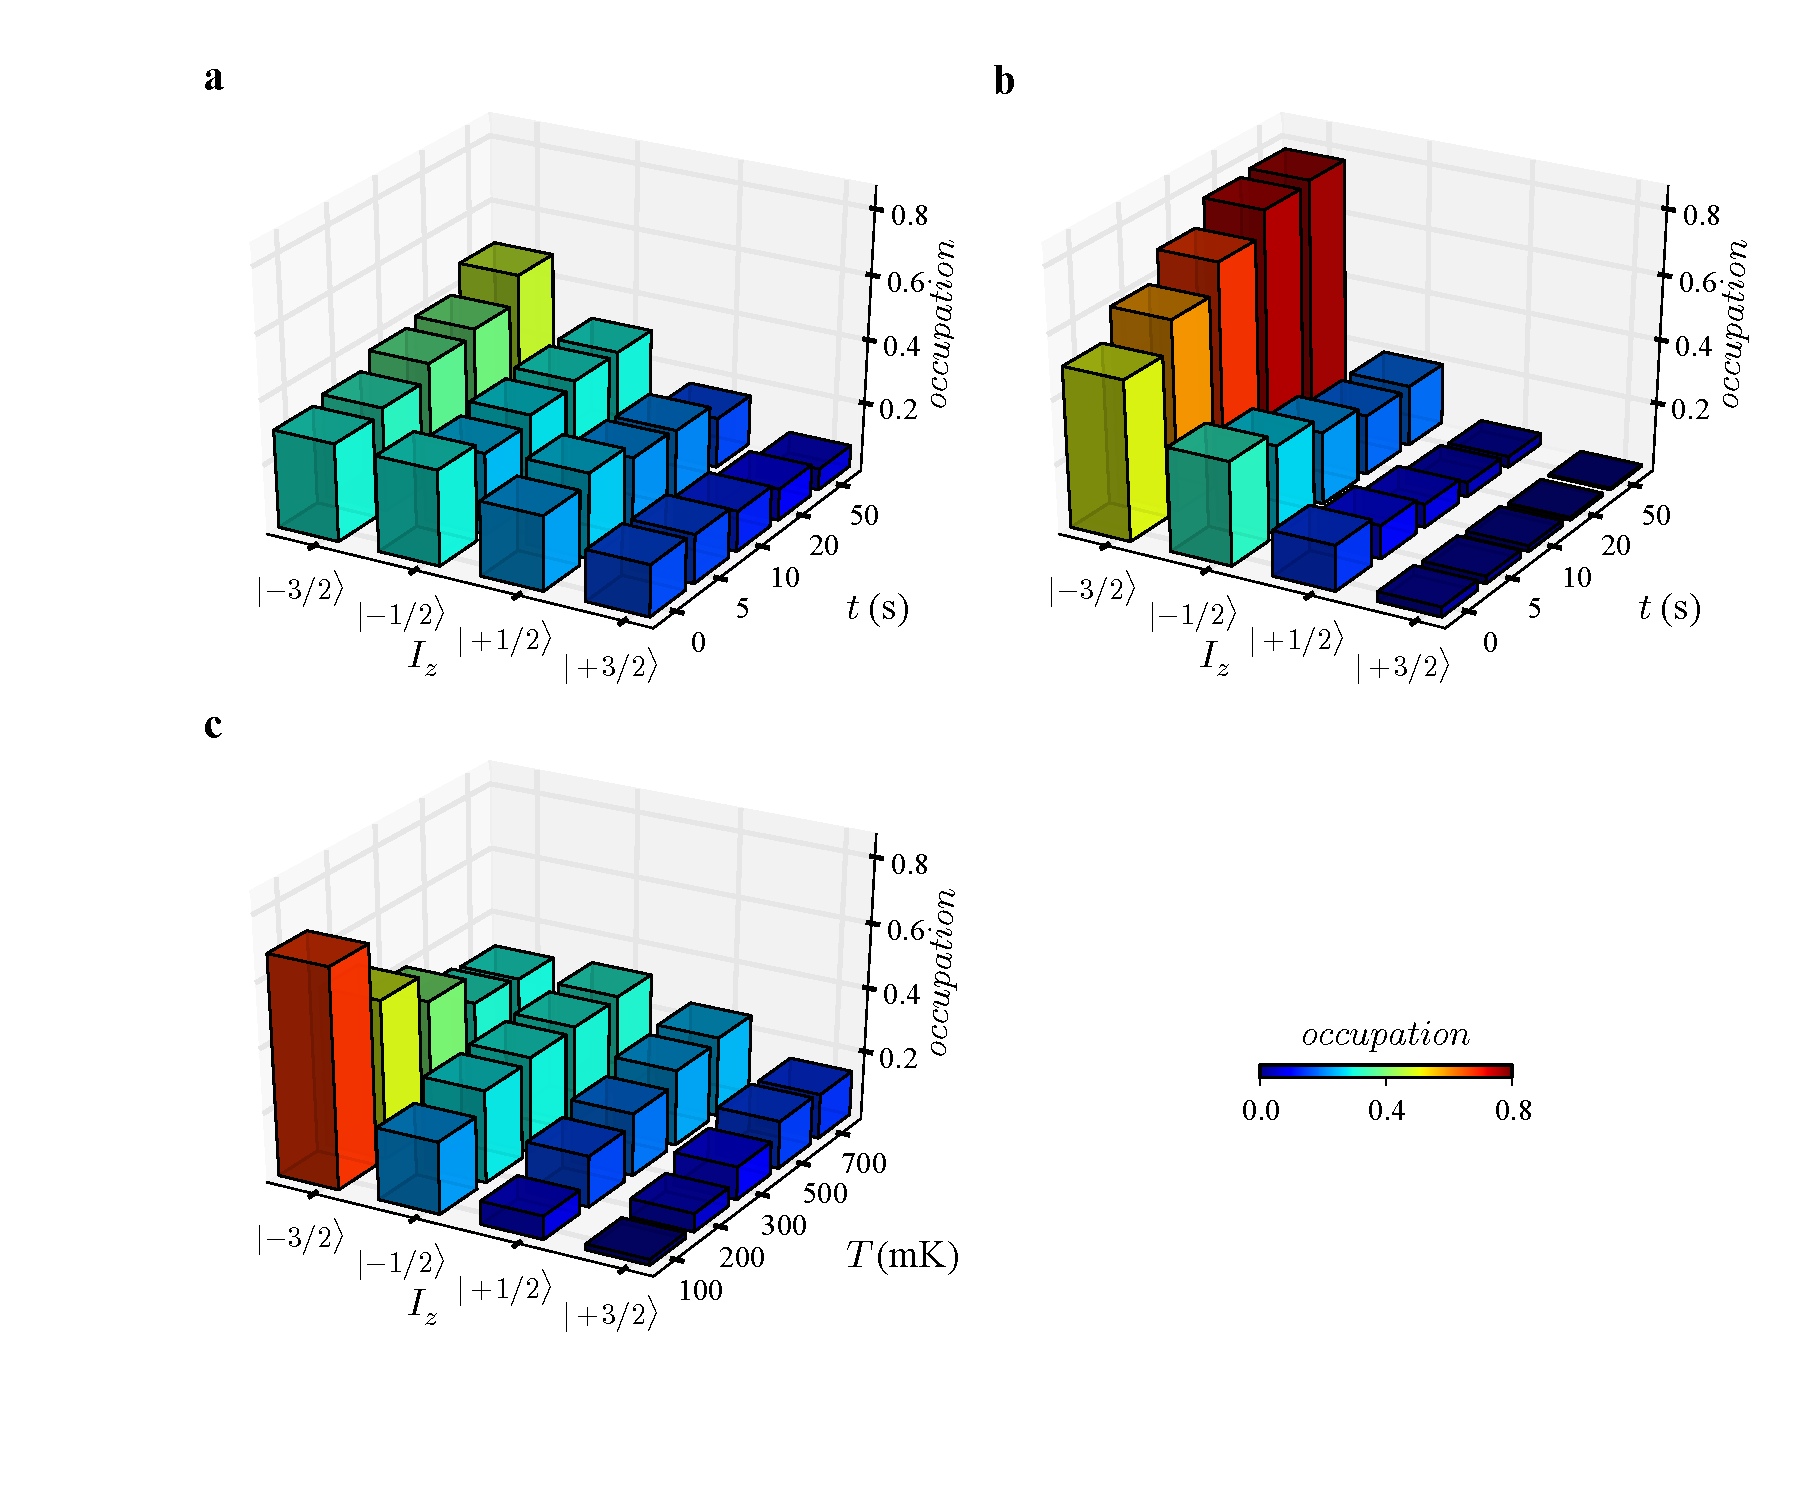
\includegraphics[scale=0.45]{Resultats/Chap2/Figure5/figure5.pdf} 
\caption{Evolution de la population des états nucléaire pour deux points de fonctionnement différent : \textbf{a}, $V_g = -0.9\,V$; et \textbf{b}, $V_g = -0.1\,V$ (avec à chaque fois $V_{ds} = 0\,V$. Ces deux mesures montrent clairement que le système évolue vers deux équilibres thermodynamique différent. \textbf{c}, dynamique du spin nucléaire pour un temps d'attente de 10 secondes, en fonction de la température $T$. Lorsque l'on augmente la température, la population des états de spin nucléaire évolue vers une occupation égale de tous les états.}
\label{dynamique_spin}
\end{figure}

\subsection{Influence de la température}

La température du spin nucléaire a également été mesuré. Pour cela, nous avons choisi de nous placer sur le second point de fonctionnement pour lequel l'équilibre est atteint plus rapidement, ce qui nous  a permis de choisir un temps d'attente relativement faible pour effectuer notre étude. En effet, au vu du nombre de mesures nécessaire (22000 mesures), on ne peut pas attendre le temps nécessaire à l'équilibre thermodynamique. Nous avons choisi un compromis en prenant un temps d'attente de 10 secondes. Bien attendu, comme le montre l'étude précédente, l'abscence d'équilibre ne nous permet pas de déduire, directement à partir de la distribution, la température du spin nucléaire.

Pour contourner cette limitation, nous avons choisi d'utiliser une méthode indirecte. Pour cela, la distribution des état nucléaire a été mesuré pour plusieurs température. La distribution observé pour $100\,mK$ a servie de référence, car celle-ci est très proche de la température électronique ($\sim 80\,mK$). La distribution ne va différé de la distribution de référence qu'à condition que la température imposé au système soit supérieur à la température nucléaire de référence obtenue à $100\,mK$.

La Fig.\ref{dynamique_spin}.\textbf{c} présente l'évolution de la distribution à $10\,$ seconde en fonction de la température. La distribution évolue entre 100 et 200$\,mK$ et celle-ci est largement modifié pour $T\geq 300mK$. Les états de plus hautes énergies commencent à se peupler pour tendre vers l'équiprobabilité vers $T=700\,mK$. On peut donc en déduire qu'à la température de base, la température d'équilibre du spin nucléaire se situe entre 100 et 200 $\,mK$, preuve que le spin nucléaire peut être refroidi de manière efficace. En effet, cette température d'équilibre est très proche de la température électronique de notre système évalué autour de $100\,mK$.